\section{HPC and QC hybridazation}

\begin{frame}{HPC and QC are natural allies}
HPC and QC are complementary from the system point of view
\begin{itemize}
    \item no Operating system runs on Quantum Computer
    \item you need some standard HPC commponents to bootstrap QC
\end{itemize}
HPC and QC are complementary as computation is concerned
\begin{itemize}
    \item QC is very good at solving NP problems
    \item some sophisticated parts of problems are easy to proceed on QC (e.g. DFT as QFT)
    \item on the other hand, some very easy operations are difficult to handle in QC (sums and products)
\end{itemize}
It's quite natural to mix HPC and QC, producing algorithms that takes benefits from both HPC and QC
\end{frame}

\begin{frame}{QAOA: the concrete example}
The \textit{Quantum Approximate Optimization Algorithm} or \textbf{QAOA} is a very classical algorithms. It's very
popular since it produces actual result even with noisy QPUs
\newline

QUBO can be solved by using Analogic Quantum Computing, for example D-Wave hardware does a quantum experiment which can be 
mapped on QUBO.
\newline

QAOA uses numerical recipies to emulates the adiabatic evolution on AQC solving QUBO, using gates based circuits
\end{frame}

\begin{frame}{Gate based QAOA in a nutshell}
From a very high-level perspective, gate based QAOA can be summarized by those steps:
\begin{itemize}
    \item discretize the adiabatic evolution into small steps
    \item for each step, 
    \begin{enumerate}
        \item build a swallow  circuit by some $\beta$ and $\gamma$ vectors
        \item get a result $\rho$ and inject inputs $(\beta, \gamma)$ and output $\rho$ into an HPC optimizer (COBYLA 
        is often used)
        \item get new parameters $(\beta', \gamma')$, reconfigure the circuit and loop to step \#1.
    \end{enumerate}    
    \item iterate until the optimizer thinks the result is precise enough
\end{itemize}
\end{frame}

\begin{frame}{Design of QAOA circuit}
The gate based circuits are involve few qubits and few gates. 

Standard one qubit rotations and CNOT gates are involved
\newline

\begin{center}
 \begin{quantikz}[thin lines]
    & \ket{a} & \ctrl{1} & \qw             & \ctrl{1} & \qw      & \qw             & \qw & \qw\\
    & \ket{b} & \targ{}  & \gate{R_Z(a.t)} & \targ{}  & \ctrl{1} & \qw             & \ctrl{1} 
    & \qw\ \\
    & \ket{c} & \qw      & \qw             & \qw      & \targ{}  & \gate{R_Z(b.t)} & \targ{} 
    & \qw\
\end{quantikz}
\end{center}    
\end{frame}

\begin{frame}{QAOA on Pasqal hardware}
In the next slides, we'll show how Rydberg atoms, on Pasqal hardware, can be used for solving QUBO.
Those slides are inspired from a Pasqal tutorial located at \url{https://pulser.readthedocs.io/en/latest/tutorials/qubo.html}
\newline

QUBO is design by a symmetric and real matrix $Q$ whose size is $N \times N$. If $z=(z_1, z_2, \cdots, z_N) \in \{0,1\}^N$, 
we can associated $Q$ with $f(z) = z^T.Q.z$.
\newline 

We want to find the minimum value for $f$. 
\end{frame}

\begin{frame}[fragile]
\frametitle{The Q matrix in our examples}
In what's follow, we will use this matrix
\begin{verbatim}
Q = np.array(
    [
        [-10.0, 19.7365809, 19.7365809, 5.42015853, 5.42015853],
        [19.7365809, -10.0, 20.67626392, 0.17675796, 0.85604541],
        [19.7365809, 20.67626392, -10.0, 0.85604541, 0.17675796],
        [5.42015853, 0.17675796, 0.85604541, -10.0, 0.32306662],
        [5.42015853, 0.85604541, 0.17675796, 0.32306662, -10.0],
    ]
)
\end{verbatim}
\end{frame}


\begin{frame}[fragile]
\frametitle{QUBO in HPC lazy mode}[fragile]
Let $Q$ be defined by a constant NumPy array (an object whose type is \texttt{np.array})
\begin{verbatim}
bitstrings = [np.binary_repr(i, len(Q)) for i in range(2 ** len(Q))]
costs = []
# this takes exponential time with the dimension of the QUBO
for b in bitstrings:
    z = np.array(list(b), dtype=int)
    cost = z.T @ Q @ z
    costs.append(cost)
zipped = zip(bitstrings, costs)
sort_zipped = sorted(zipped, key=lambda x: x[1])
print(sort_zipped[:3])    
\end{verbatim}

This solves QUBO... but the elapsed time is $O(2^N)$

We find that $01011$ and $00111$ are the optimal solutions
\end{frame}


\begin{frame}{Using the Rydberg Hamiltonian}
The Pasqal hardware is based on the Rydberg interaction whose hamiltonian is 
\begin{equation*}
    H = \sum_{i=1}^N \frac{\hbar\Omega}{2}\sigma_i^x - \sum_{i=1}^N \frac{\hbar\delta}{2}\sigma_i^z +
        \sum_{j < i}\frac{C_6}{|r_i - r_j|^6}n_i n_j
\end{equation*}
Pulser makes it possible to put atoms at known location on a lattice, one of the term depends on the pairwise distance 
betweeen two atoms $U = \frac{C_6}{|r_i - r_j|^6}$. 
\newline

In this step, we embed the QUBO onto an atomic register. The resulting hamiltonian $H_Q$ will have a ground state
corresponding to the minimum value of $f(z) = z^T.Q.z$ 
\end{frame}

\begin{frame}[fragile]
\frametitle{Embedding a QUBO onto an atomic register 1/2}  
\begin{small}
\begin{verbatim}
def evaluate_mapping(new_coords, *args):
    """Cost function to minimize. Ideally, the pairwise
    distances are conserved"""
    Q, shape = args
    new_coords = np.reshape(new_coords, shape)
    new_Q = squareform(
        DigitalAnalogDevice.interaction_coeff / pdist(new_coords) ** 6
    )
    return np.linalg.norm(new_Q - Q)

\end{verbatim}
\end{small}
\end{frame}


\begin{frame}[fragile]
\frametitle{Embedding a QUBO onto an atomic register 2/2}  
\begin{small}
\begin{verbatim}
shape = (len(Q), 2)
costs = []
np.random.seed(0)
x0 = np.random.random(shape).flatten()
res = minimize(
    evaluate_mapping,
    x0,
    args=(Q, shape),
    method="Nelder-Mead",
    tol=1e-6,
    options={"maxiter": 200000, "maxfev": None},
)
coords = np.reshape(res.x, (len(Q), 2))
\end{verbatim}
\end{small}
\end{frame}

\begin{frame}{Resulting atoms grid}
The result is this atoms grid
\begin{center}
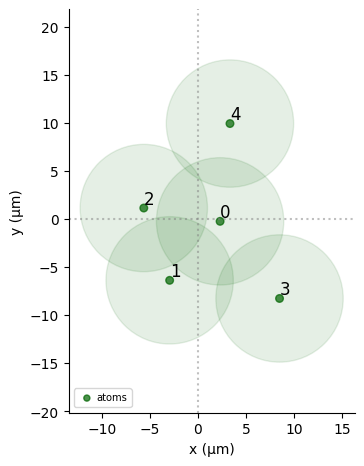
\includegraphics[height=7cm]{images/tutorials_qubo_14_0.png}    
\end{center}
\end{frame}



\begin{frame}{Moving the atoms to emulate QUBO}
We will use the \textit{Rydberg representation} of an hamiltonian by
\begin{itemize}
    \item we start is the state $H_I$ where $\Omega = 1 rad/{\mu s}$ and $\delta = 0 rad/{\mu s}$ 
    \item we end in the state $H_Q$ where  $\Omega = 0 rad/{\mu s}$ and $\delta = 1 rad/{\mu s}$ 
    \item we build parameterized \texttt{sequence} (Pulser experiment) to move slowly from $H_I$ to $H_Q$
\end{itemize}
\end{frame}

\begin{frame}[fragile]
\frametitle{Parameterized sequence}
\begin{verbatim}
LAYERS = 2

# Parametrized sequence
seq = Sequence(reg, DigitalAnalogDevice)
seq.declare_channel("ch0", "rydberg_global")

t_list = seq.declare_variable("t_list", size=LAYERS)
s_list = seq.declare_variable("s_list", size=LAYERS)

for t, s in zip(t_list, s_list):
    pulse_1 = Pulse.ConstantPulse(1000 * t, 1.0, 0.0, 0)
    pulse_2 = Pulse.ConstantPulse(1000 * s, 0.0, 1.0, 0)

    seq.add(pulse_1, "ch0")
    seq.add(pulse_2, "ch0")

seq.measure("ground-rydberg")    
\end{verbatim}
\end{frame}

\begin{frame}[fragile]
\frametitle{looping on sequences}
\begin{verbatim}
def quantum_loop(parameters):
    params = np.array(parameters)
    t_params, s_params = np.reshape(params.astype(int), (2, LAYERS))
    assigned_seq = seq.build(t_list=t_params, s_list=s_params)
    simul = QutipEmulator.from_sequence(assigned_seq, sampling_rate=0.01)
    results = simul.run()
    count_dict = results.sample_final_state()  # sample from the state vector
    return count_dict

np.random.seed(123)  # ensures reproducibility of the tutorial
guess = {
    "t": np.random.uniform(8, 10, LAYERS),
    "s": np.random.uniform(1, 3, LAYERS),
}    
example_dict = quantum_loop(np.r_[guess["t"], guess["s"]])


\end{verbatim}    
\end{frame}

\begin{frame}{looping on sequences and getting results}
A first run of function \texttt{quantum\_loop}, without optimisation, gets this resukt
\begin{center}
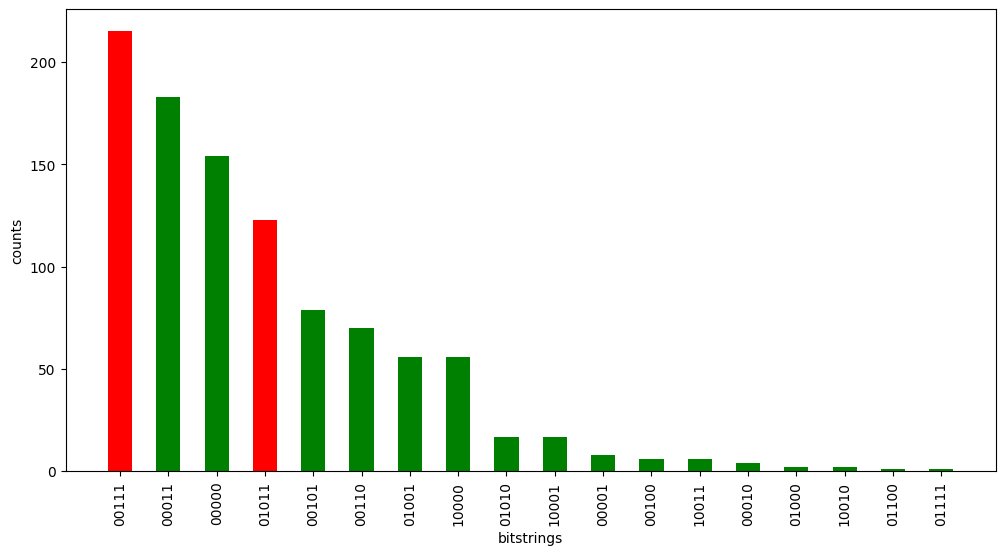
\includegraphics[width=8cm]{images/tutorials_qubo_27_0.png}    
\end{center}
We know that $01011$ and $00111$ are two minimal solution. We have not yet converged
\end{frame}

\begin{frame}[fragile]
\frametitle{Performing the optimisation}
A cost function \texttt{get\_cost}, computing $z^T.Q.z$ is define, it is fully polynomial. 

It it wrapped with  with \texttt{quantum\_loop}
\begin{verbatim}

def get_cost(counter, Q):
    cost = sum(counter[key] * get_cost_colouring(key, Q) for key in counter)
    return cost / sum(counter.values())  # Divide by total samples
    
def func(param, *args):
    Q = args[0]
    C = quantum_loop(param)
    cost = get_cost(C, Q)
    return cost    
\end{verbatim}
\end{frame}

\begin{frame}[fragile]
\frametitle{Invokation of the HPC optimizer}
\begin{verbatim}
scores = []
params = []
(...)
    try:
        res = minimize(
            func,
            args=Q,
            x0=np.r_[guess["t"], guess["s"]],
            method="Nelder-Mead",
            tol=1e-5,
            options={"maxiter": 10},
        )
        scores.append(res.fun)
        params.append(res.x)
(...)
\end{verbatim}    
\end{frame}


\begin{frame}{looping on sequences and getting results}
 
\begin{center}
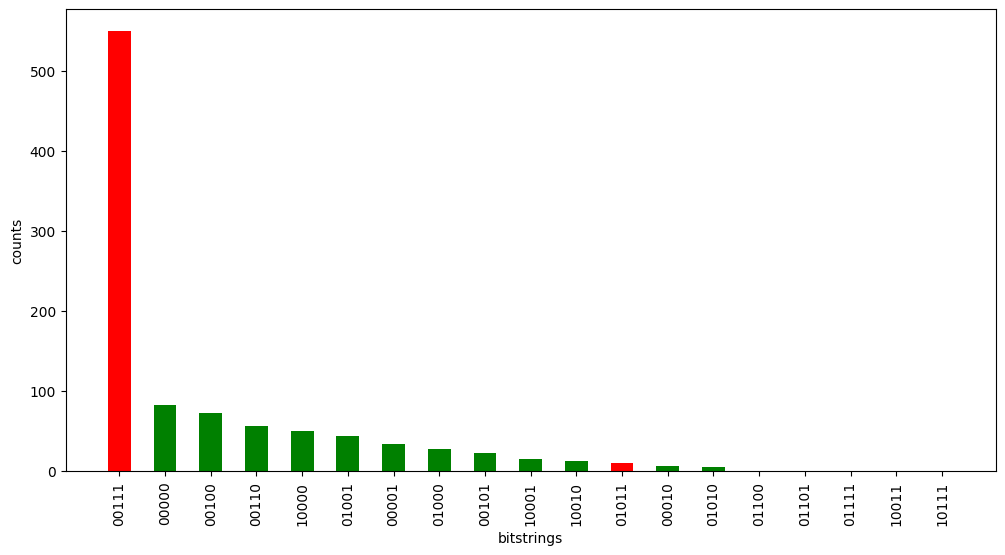
\includegraphics[width=8cm]{images/tutorials_qubo_38_0.png}    
\end{center}
Known solution are in red, we've found one, but thes second is still hidden. 
 
\end{frame}

\begin{frame}{The adiabatic theorem for dummies}
In Quantum Physics theory the adiabatic theorem says (roughly...)
\begin{itemize}
    \item a system is at the ground state of a system whose Hamiltonian $H_I$
    \item you make this system evolve continuously and \textit{kindly} to go to a configuration described by 
    hamiltonian $H_F$
    \item this evolution is \textbf{adiabatic}; no energy is brought to the system
\end{itemize}
Well... if you were nice enough with the system, you took it from $H_I$ in its ground state and put it $H_F$, at the 
ground state of $H_F$.

By measuring the state, you know what the ground state of $H_F$ is !!
This is (very roughly) how D-Wave machines operate. 
\newline
Let's build a sequence that make $\Omega$ and $\delta$ evolve adiabatically. 
\end{frame}


\begin{frame}[fragile]
\frametitle{Related Pulser code}
\begin{verbatim}
# We choose a median value between the min and the max
Omega = np.median(Q[Q > 0].flatten())
delta_0 = -5  # just has to be negative
delta_f = -delta_0  # just has to be positive
T = 4000  # time in ns, we choose a time long enough to ensure the propagation of information in the system

adiabatic_pulse = Pulse(
    InterpolatedWaveform(T, [1e-9, Omega, 1e-9]),
    InterpolatedWaveform(T, [delta_0, 0, delta_f]),
    0,
)
seq = Sequence(reg, DigitalAnalogDevice)
seq.declare_channel("ising", "rydberg_global")
seq.add(adiabatic_pulse, "ising")
seq.draw()
\end{verbatim}
\end{frame}
\begin{frame}{Adiabatic evolution}
We evolution of $\Omega$ and $\delta$ wavelengths will be design like this
\begin{center}
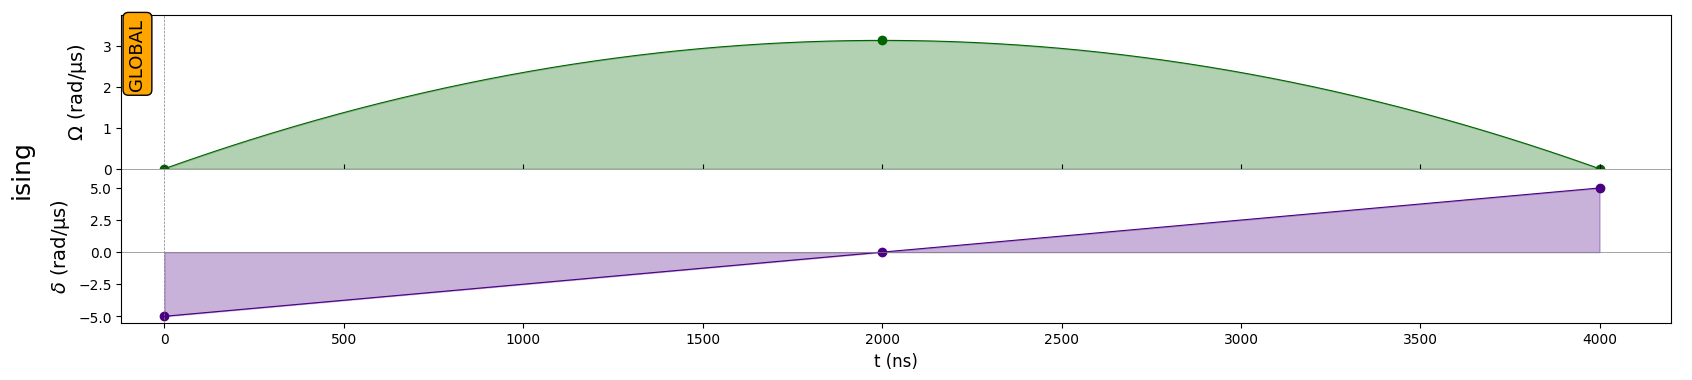
\includegraphics[width=14cm]{images/tutorials_qubo_46_0.png}    
\end{center}
\end{frame}

\begin{frame}{looping on sequences and getting results}
This time, we find both solutions in a very fast way 
\begin{center}
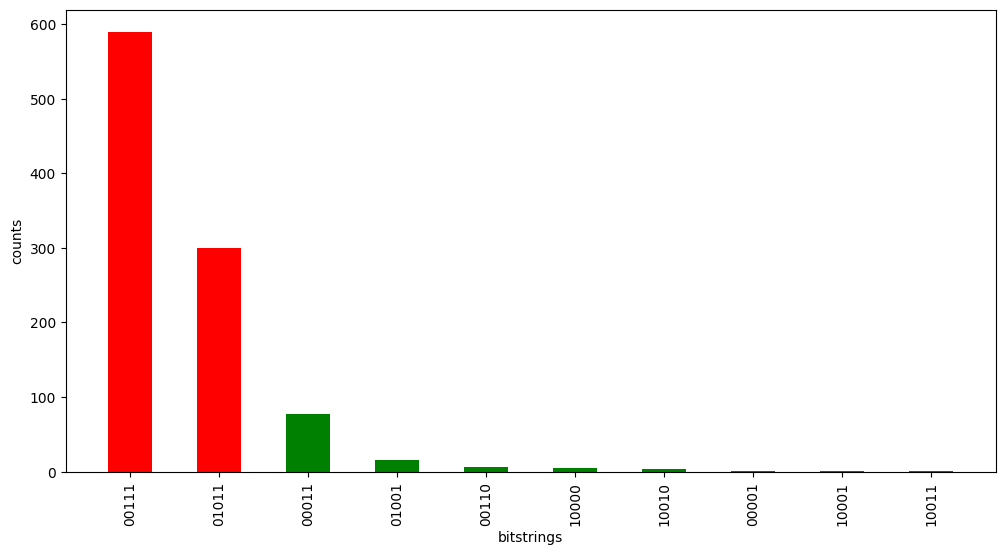
\includegraphics[width=8cm]{images/tutorials_qubo_48_0.png}    
\end{center}
It worked fine with this example, but building a $(\Omega, \delta)$ adiabatic evolution is complex.
 
\end{frame}